\subsection{集群运行}
经过多次实验的证实,我们确认我们的程序可以在集群上运行并输出正确结果。
我们最后一次实验在集群的Yarn WebUI上的运行报告截图如下:
\\
\emph{注:任务6的实现已包含在任务4和任务5的实现中}
% \begin{figure}[ht]
% \centering
% \subfigure[任务1:人物名分词]{
% 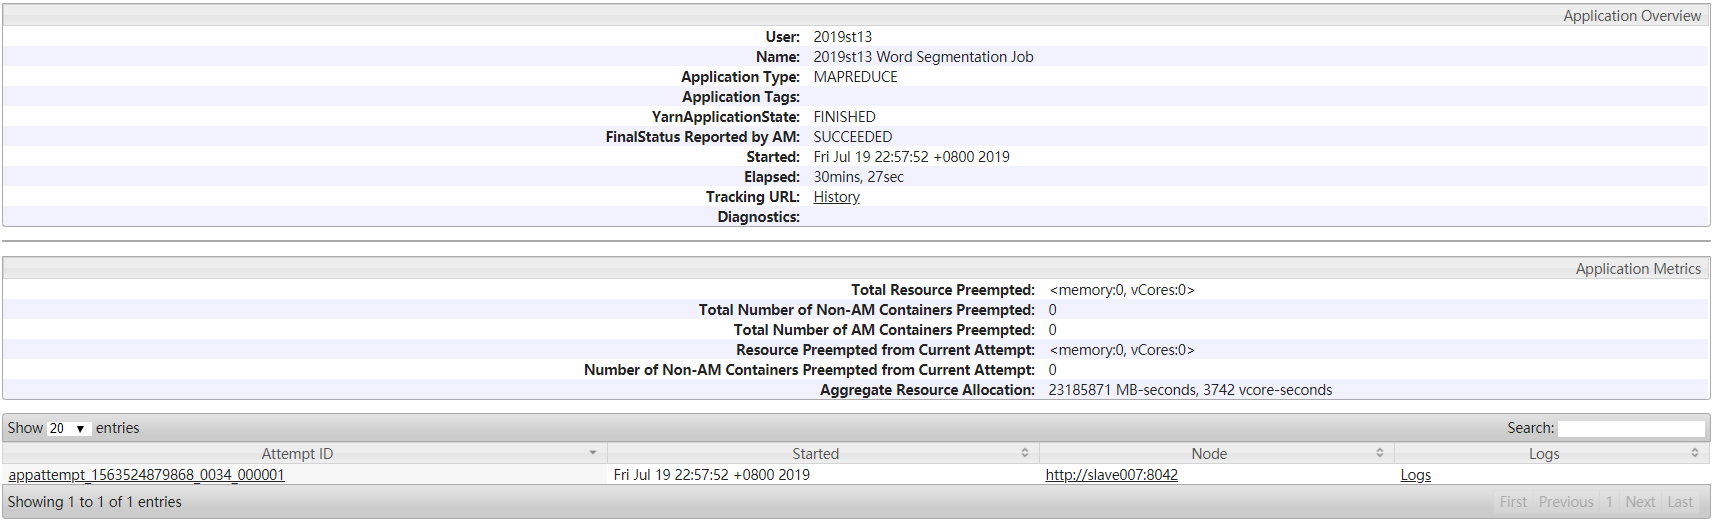
\includegraphics[scale=0.3]{figures/task1.PNG}
% }
% \subfigure[任务2:单词同现]{
% 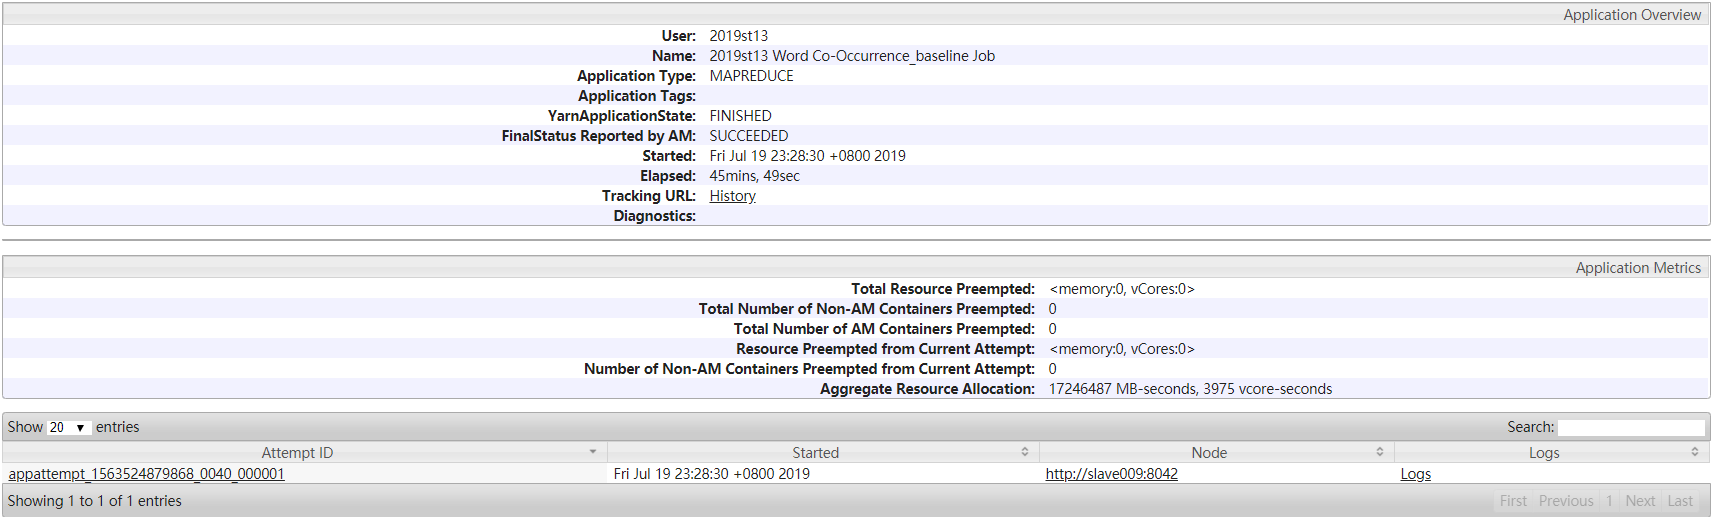
\includegraphics[scale=0.3]{figures/task2.PNG}
% }
% \subfigure[任务3:归一化]{
% 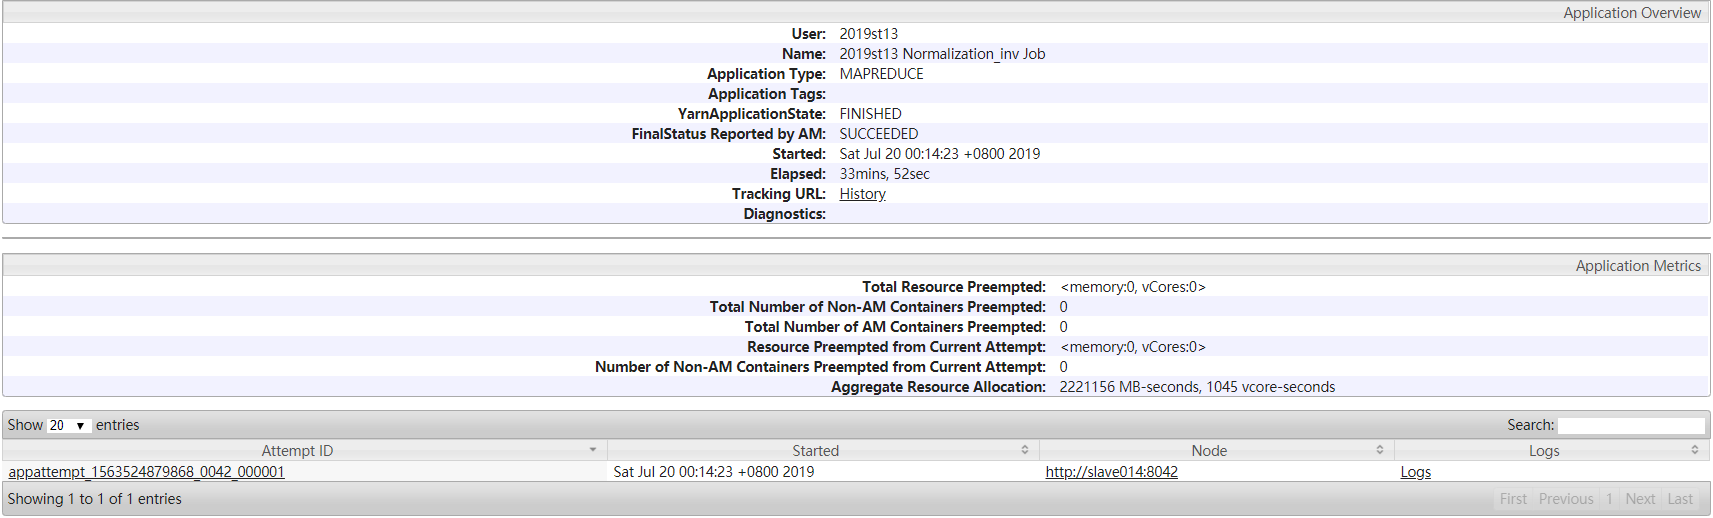
\includegraphics[scale=0.3]{figures/task3.PNG}
% }
% \subfigure[任务4:PageRank]{
% 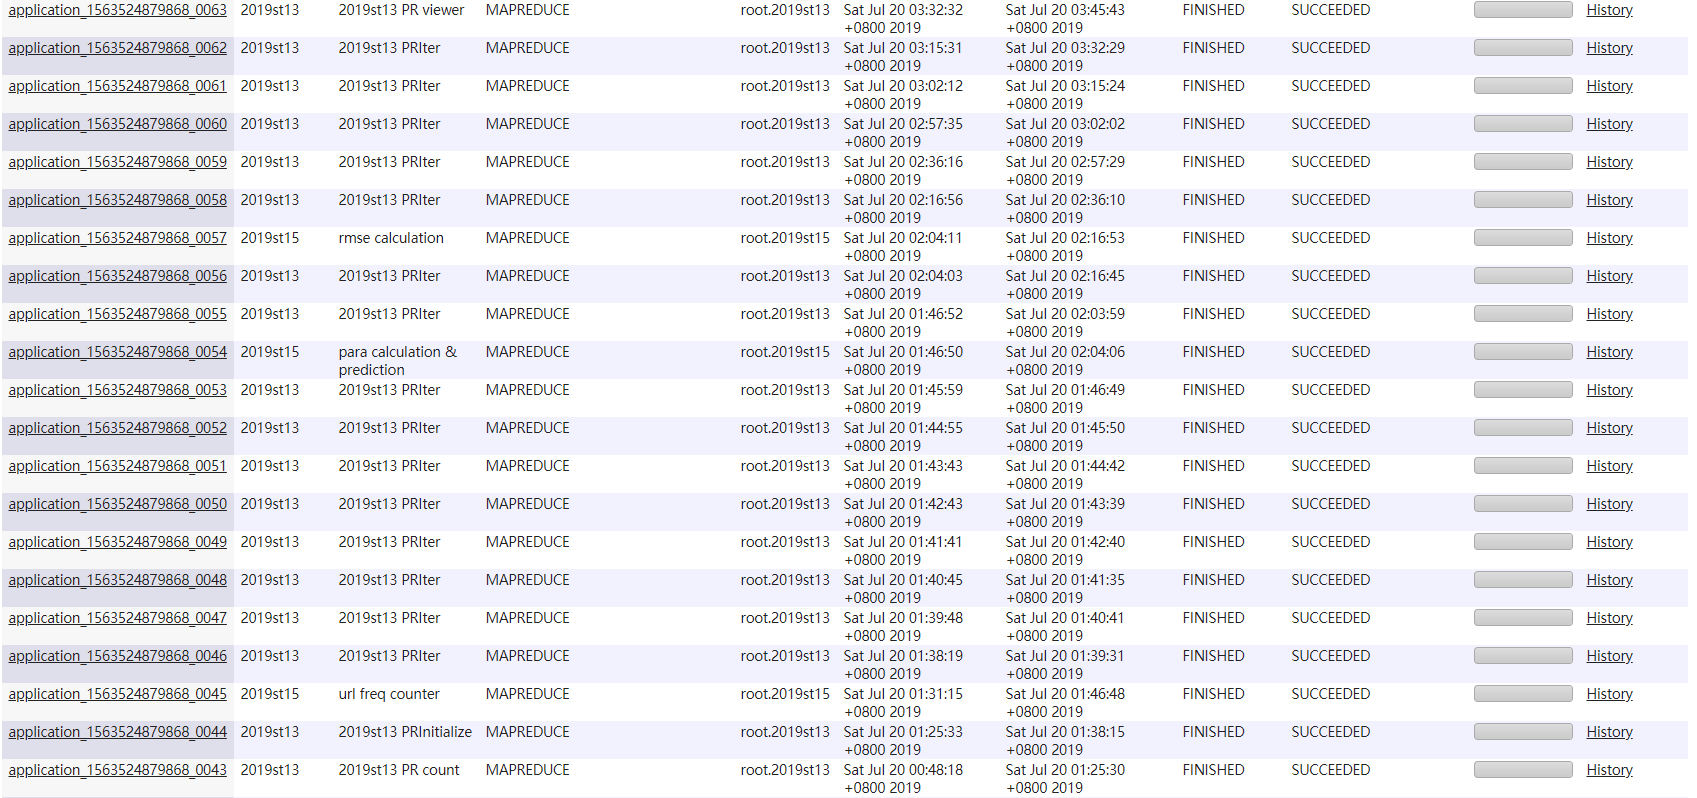
\includegraphics[scale=0.3]{figures/task4.PNG}
% }
% \subfigure[任务5:LabelPropagation]{
% 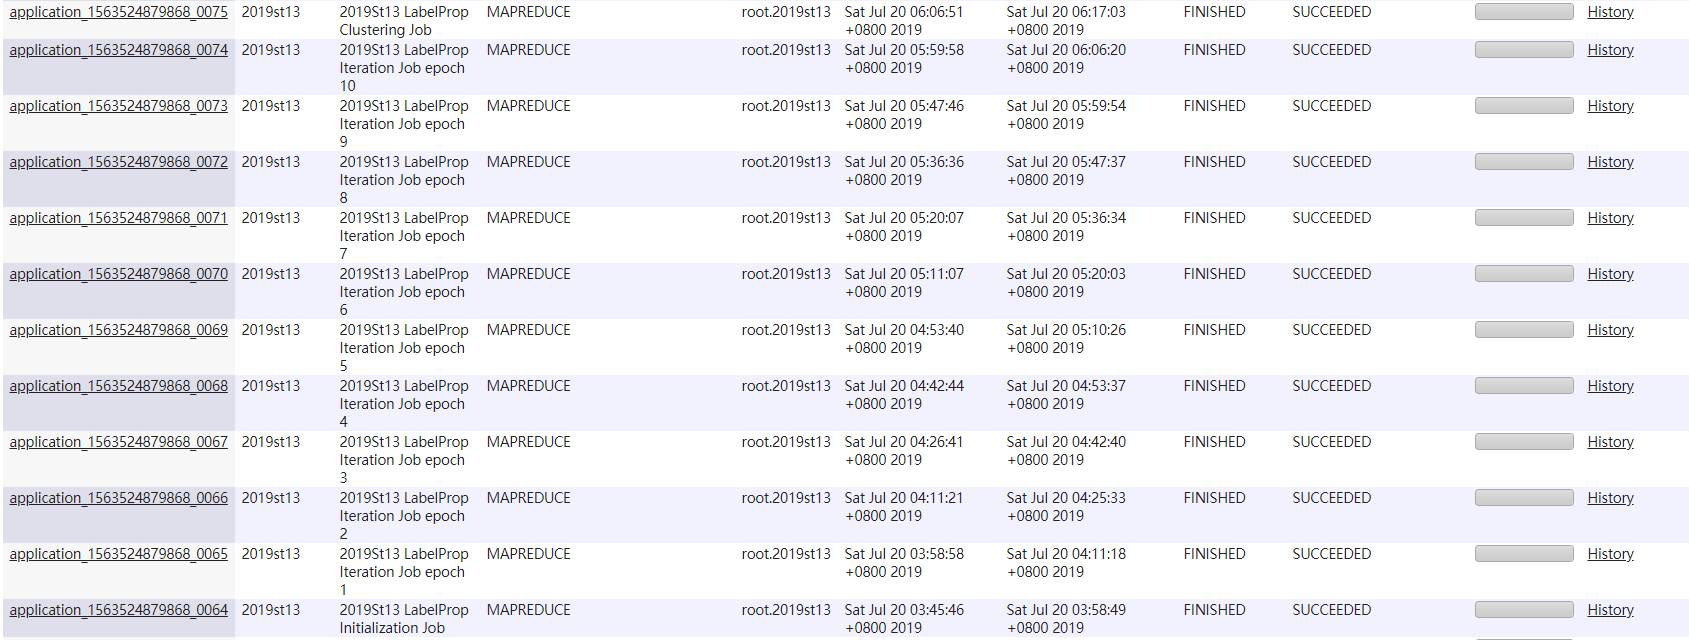
\includegraphics[scale=0.3]{figures/task5.PNG}
% }
% \caption{Yarn WebUI作业运行报告截图}
% \end{figure}
\begin{figure}[htbp]
	\centering
	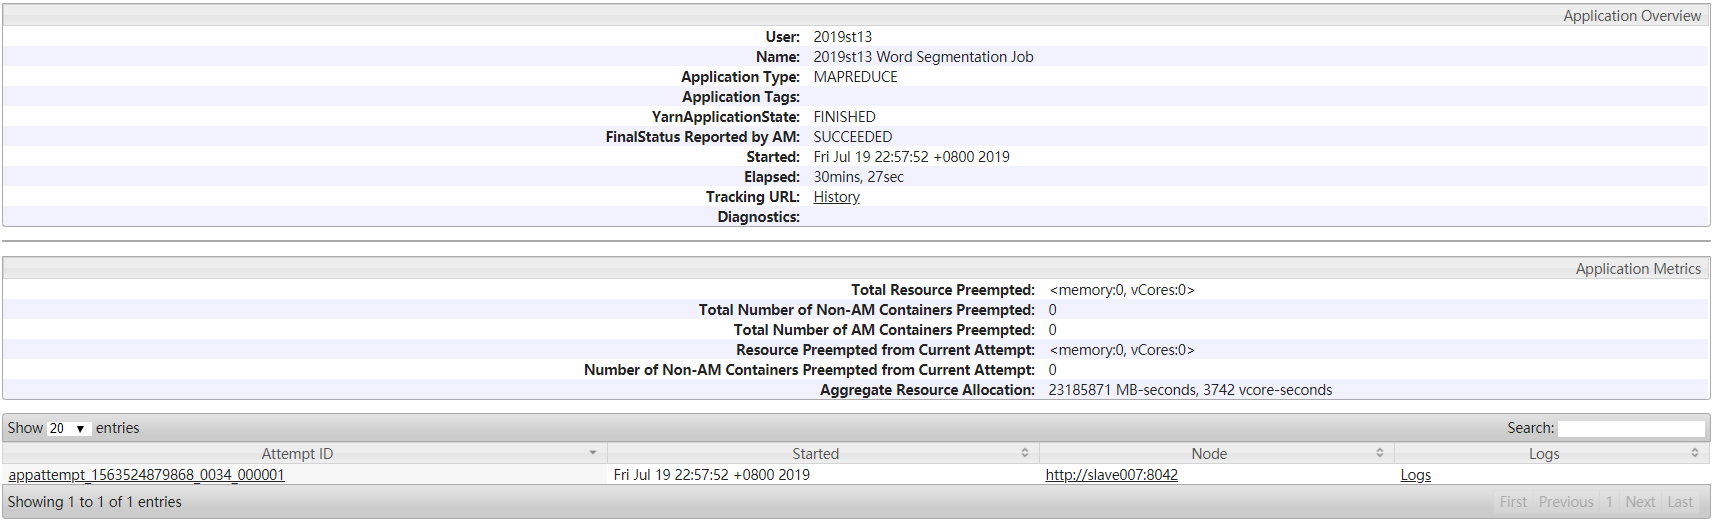
\includegraphics[scale=0.35]{figures/task1.PNG}
	\caption{任务1 人物名分词}
\end{figure}
\begin{figure}[htbp]
	\centering
	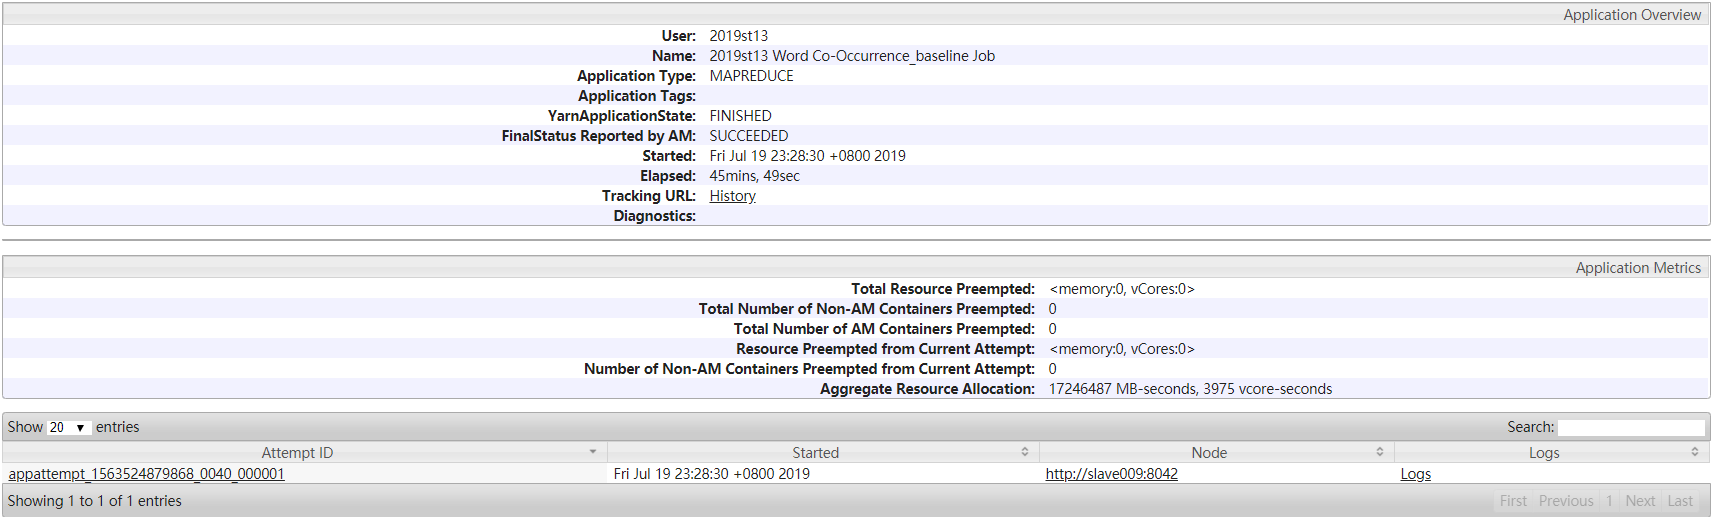
\includegraphics[scale=0.35]{figures/task2.PNG}
	\caption{任务2 单词同现}
\end{figure}
\begin{figure}[htbp]
	\centering
	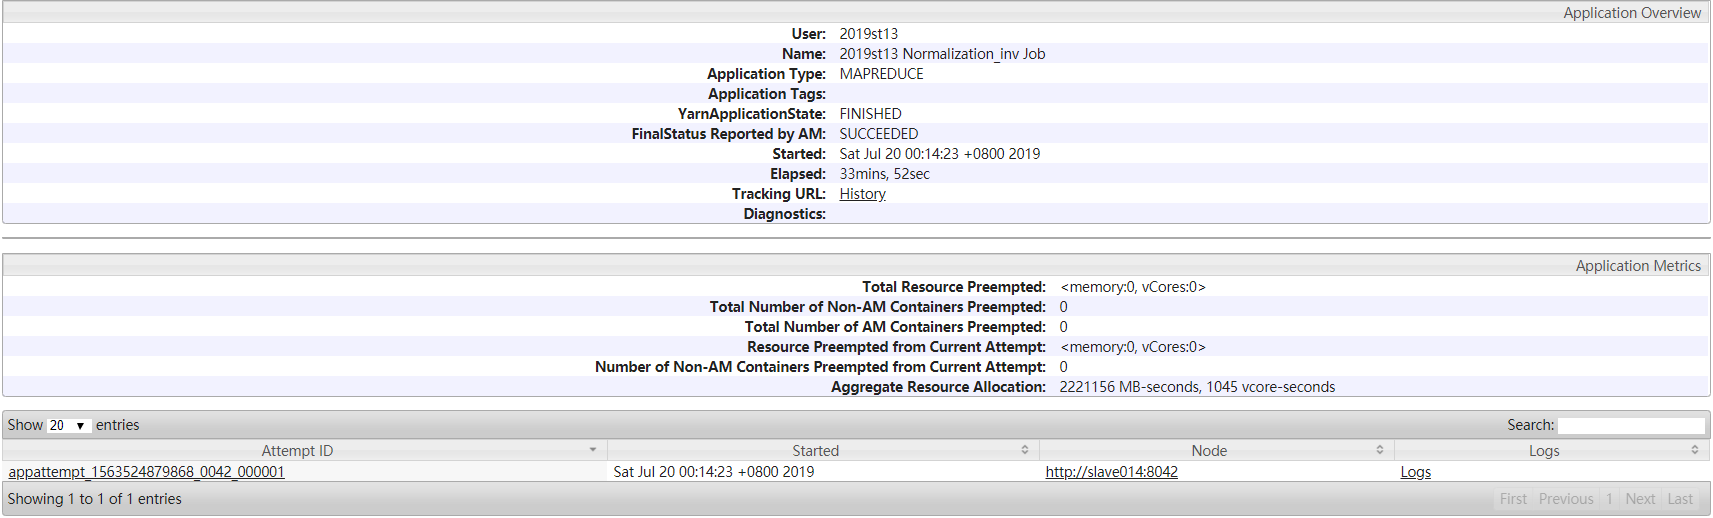
\includegraphics[scale=0.35]{figures/task3.PNG}
	\caption{任务3 归一化}
\end{figure}
\begin{figure}[htbp]
	\centering
	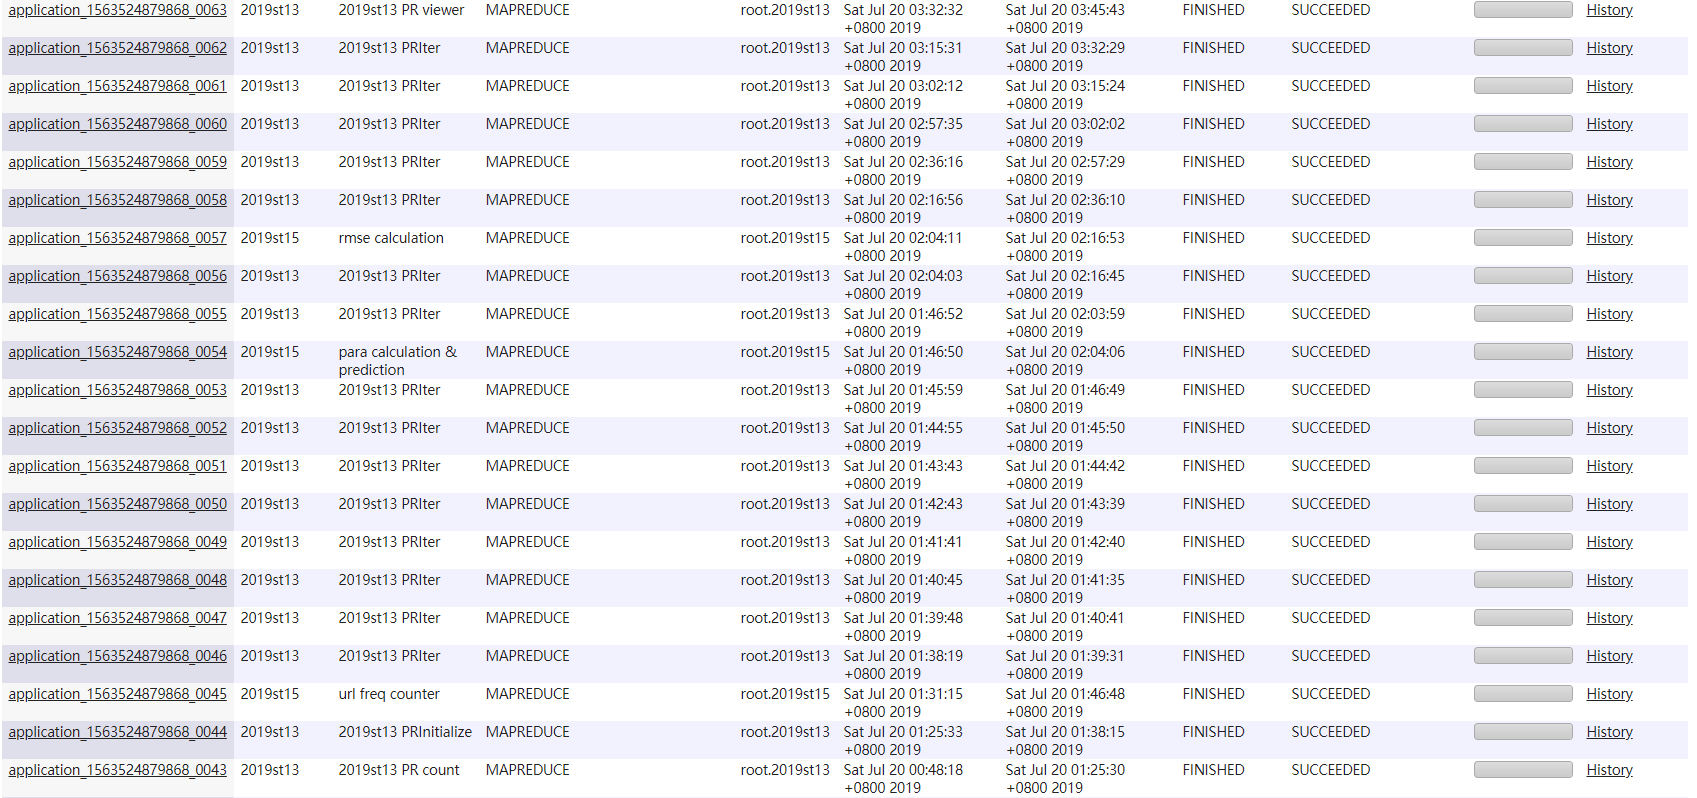
\includegraphics[scale=0.35]{figures/task4.PNG}
	\caption{任务4 PageRank}
\end{figure}
\begin{figure}[htbp]
	\centering
	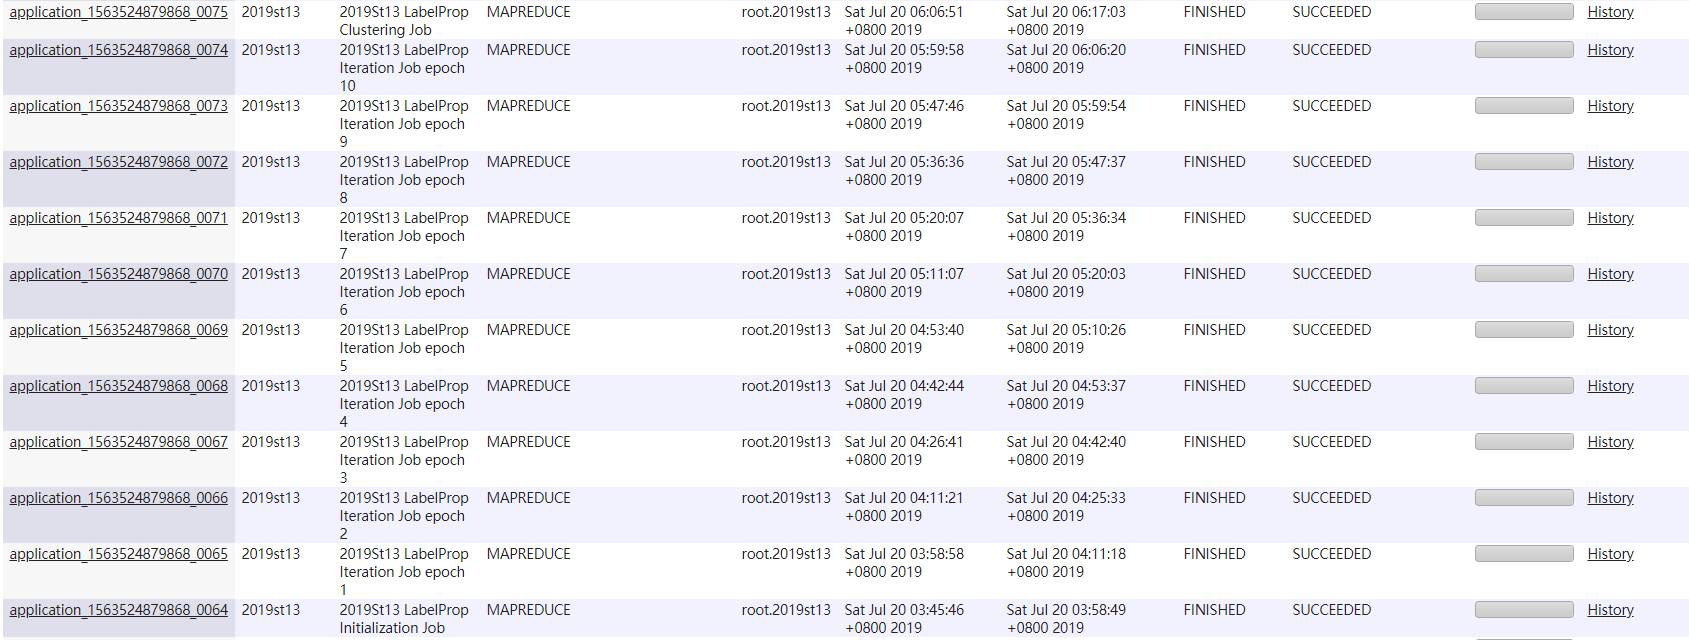
\includegraphics[scale=0.35]{figures/task5.PNG}
	\caption{任务5 LabelPropagation}
\end{figure}

\newpage
\newpage
\subsection{PageRank词云}
根据PageRank的结果,按照人物的PR值大小生成词云,可以直观的看出哪些人物是主角。
\begin{figure}[ht]
	\centering
	
\includegraphics[scale=0.38]{figures/wordcloud.jpg}
	\caption{根据PageRank值生成词云}
\end{figure}

\newpage
\subsection{标签传播聚类}
根据PageRank和标签传播的结果,对人物关系图进行染色,可以看出哪些人物之间的关系密切,哪些人物属于同一本书。
\begin{figure}[ht]
	\centering
	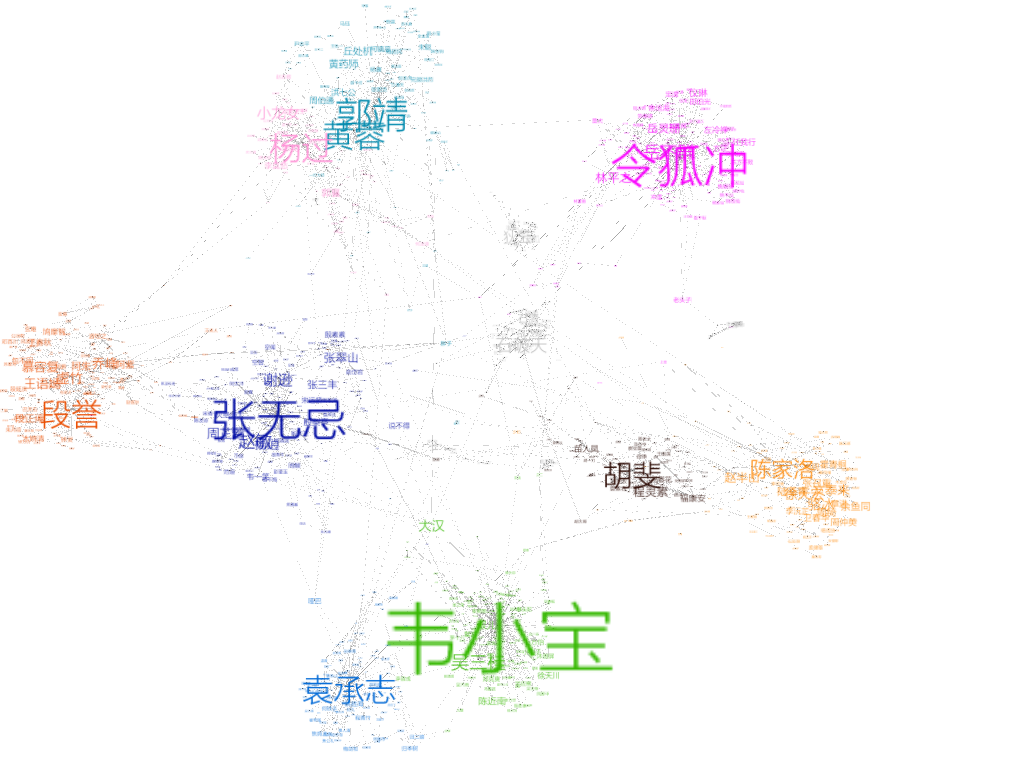
\includegraphics[scale=0.45]{figures/label_prop.png}
	\caption{标签传播结果可视化}
\end{figure}